\chapter{Guidance Assessment}\label{Ch:NumericalAssessment}

\section{Reference Trajectory Optimization}
In this section we solve the ROGP for a variety of objective weights $(w_h,\,w_s)$ while holding the gains constant. This demonstrates the extent to which the reference trajectory can impact the solution for a fixed set of gains. In the first subsection, we consider the open-loop ($K=\zero$) scenario to gauge the level of dispersions that must be mitigated by the guidance, and the extent to which open-loop shaping can help. MSL performed a similar exercise \cite{MSL_EDL2}. The second subsection repeats the sweep over the weights in a closed-loop scenario.
\subsection{Open-Loop Optimization}
\begin{figure}[h!]
	\centering
	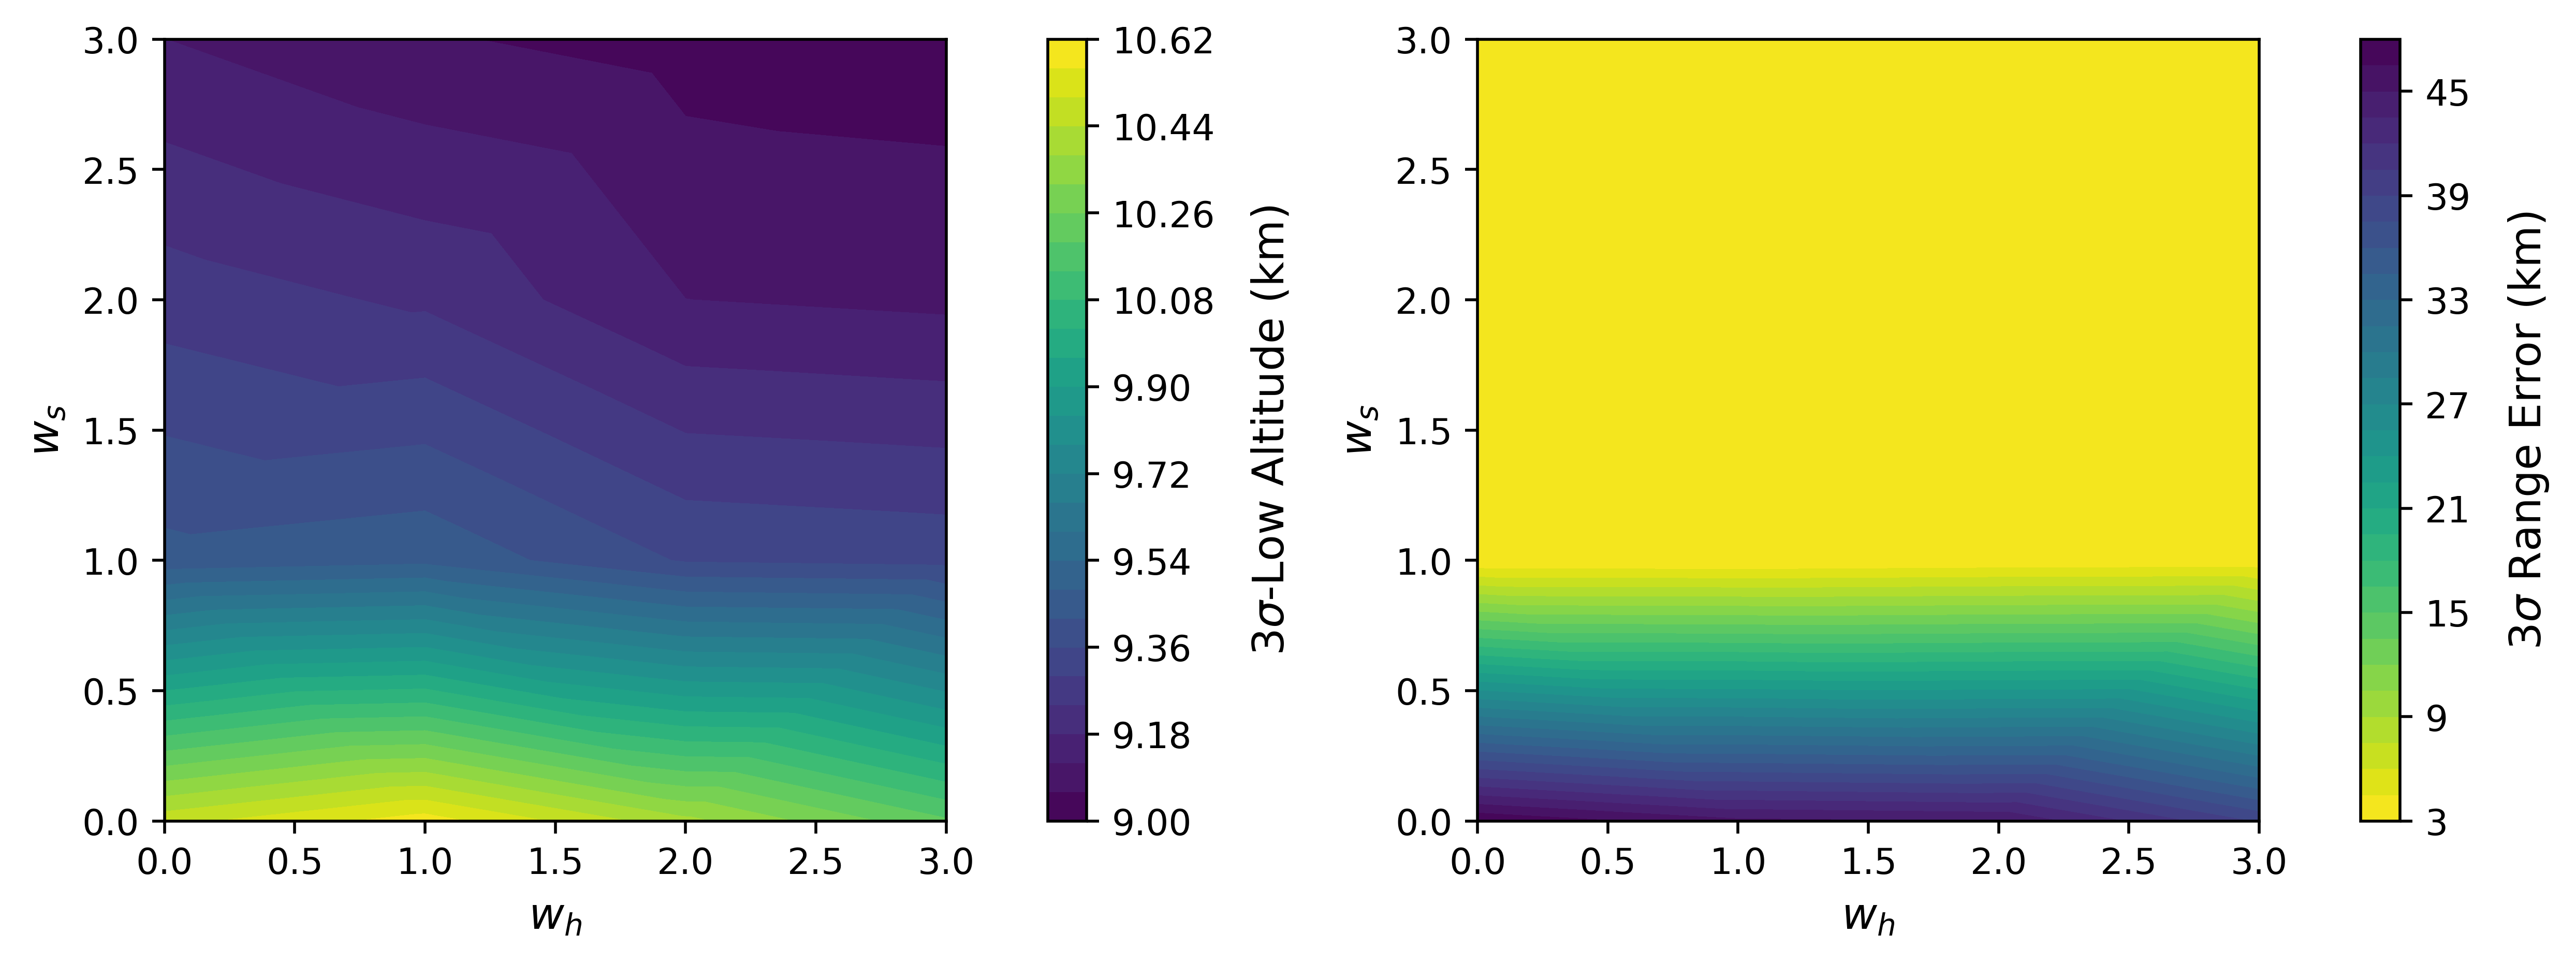
\includegraphics[width=1\textwidth]{Images/Reoptimized_WeightSweepMCResults}
	\caption{}
	\label{Fig:MCResultsOpenLoop}
\end{figure}
%\begin{figure}[h!]
%	\centering
%	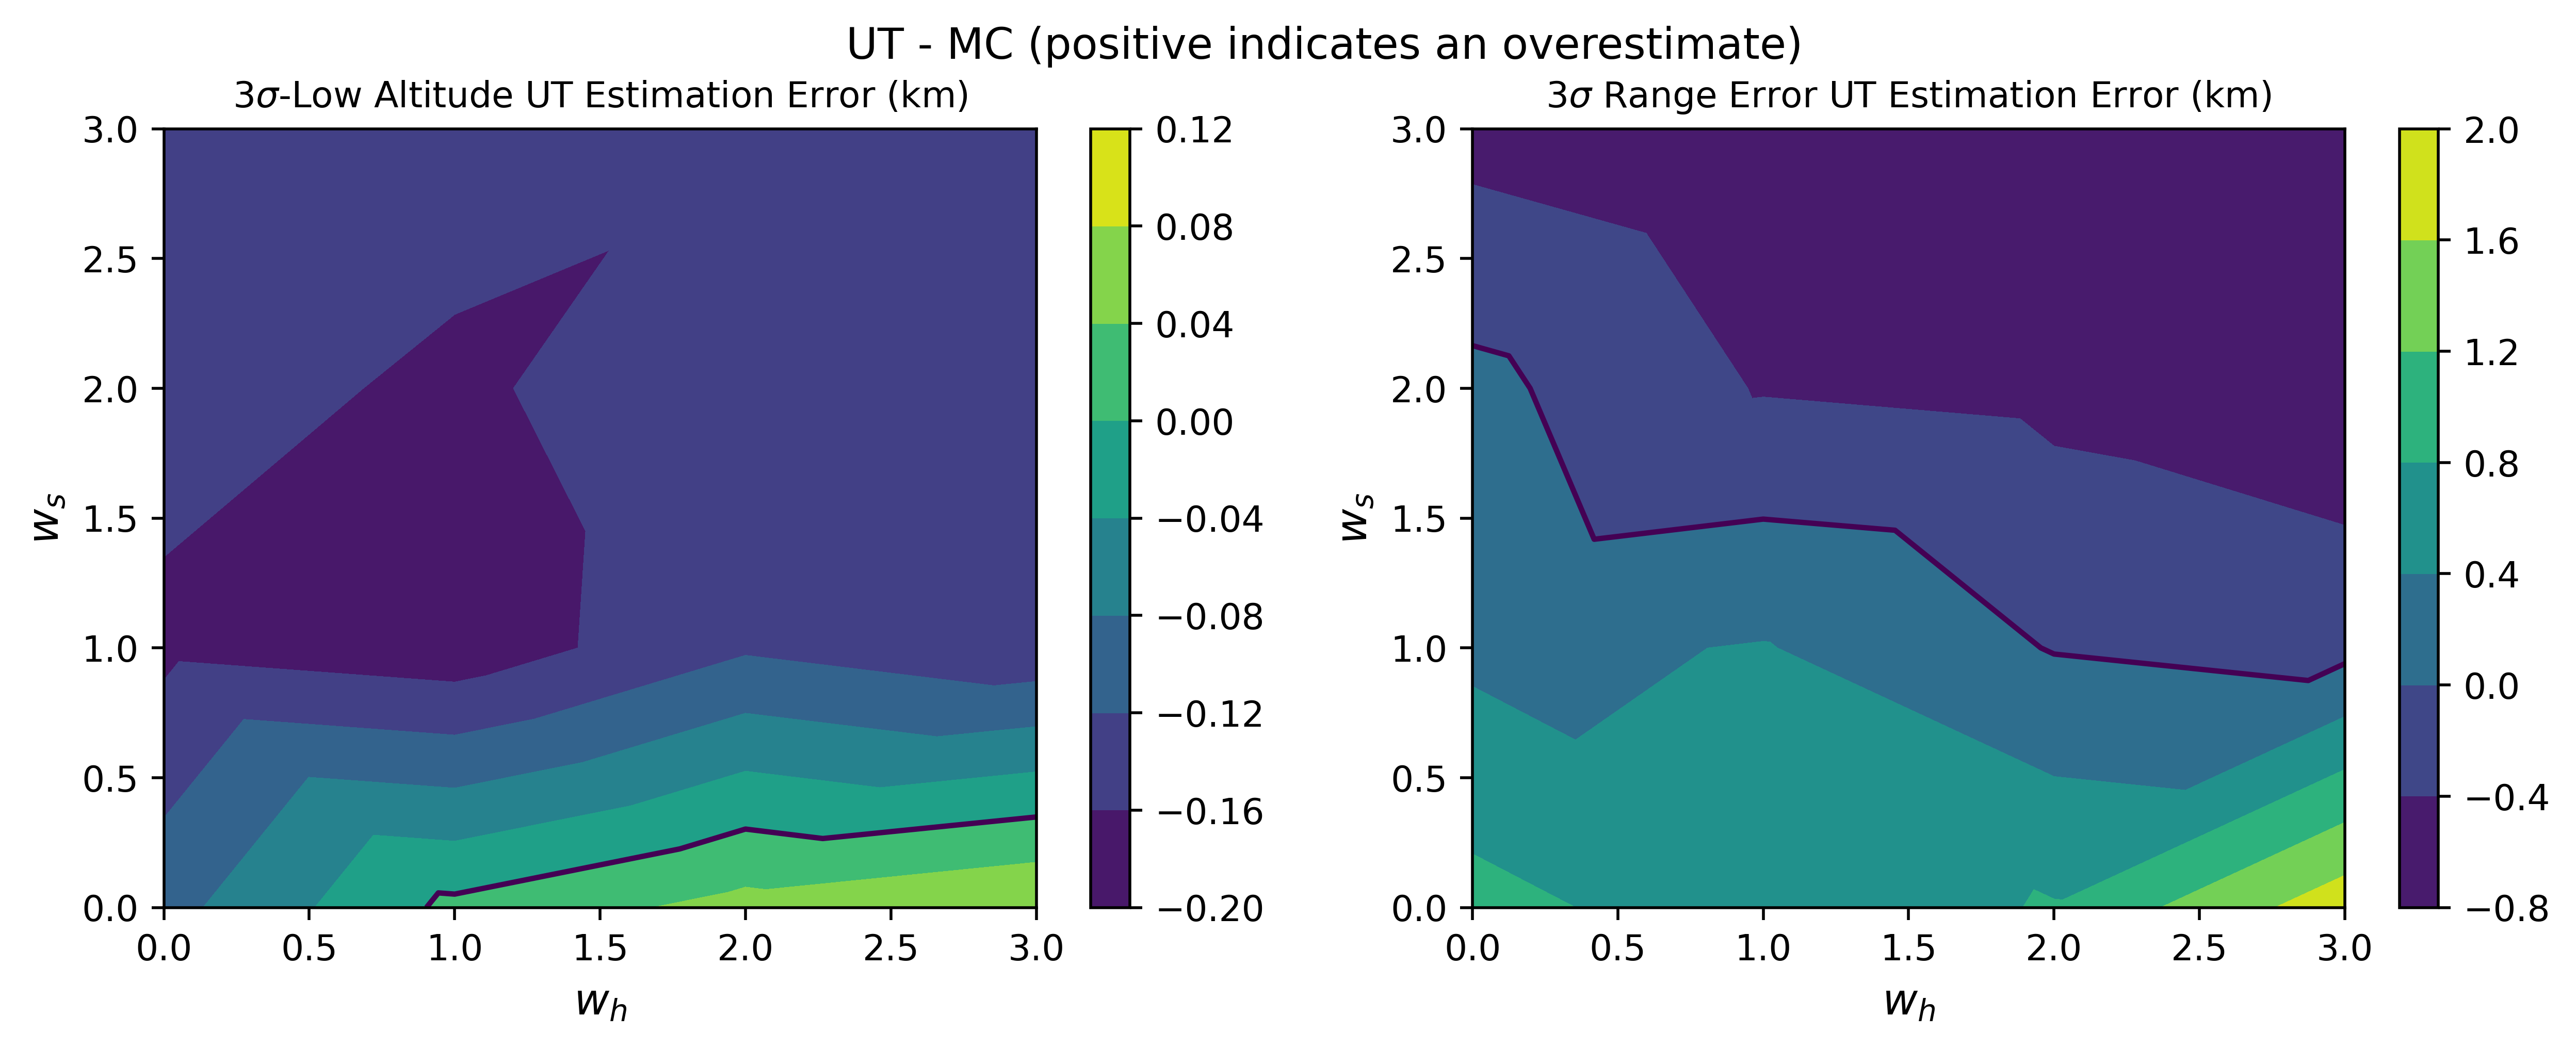
\includegraphics[width=1\textwidth]{Images/Reoptimized_WeightSweepError}
%	\caption{}
%	\label{Fig:MCErrorsOpenLoop}
%\end{figure}

\subsection{Closed-Loop Optimization}
%Maybe show ONLY  Monte Carlo results here. Then in the next section, do a detailed comparison. Justified by the fact that optimized gains are what we would want to use, so we should confirm those? But MC here already confirms. We could maybe get away with showing the UT only
\begin{figure}[h!]
	\centering
	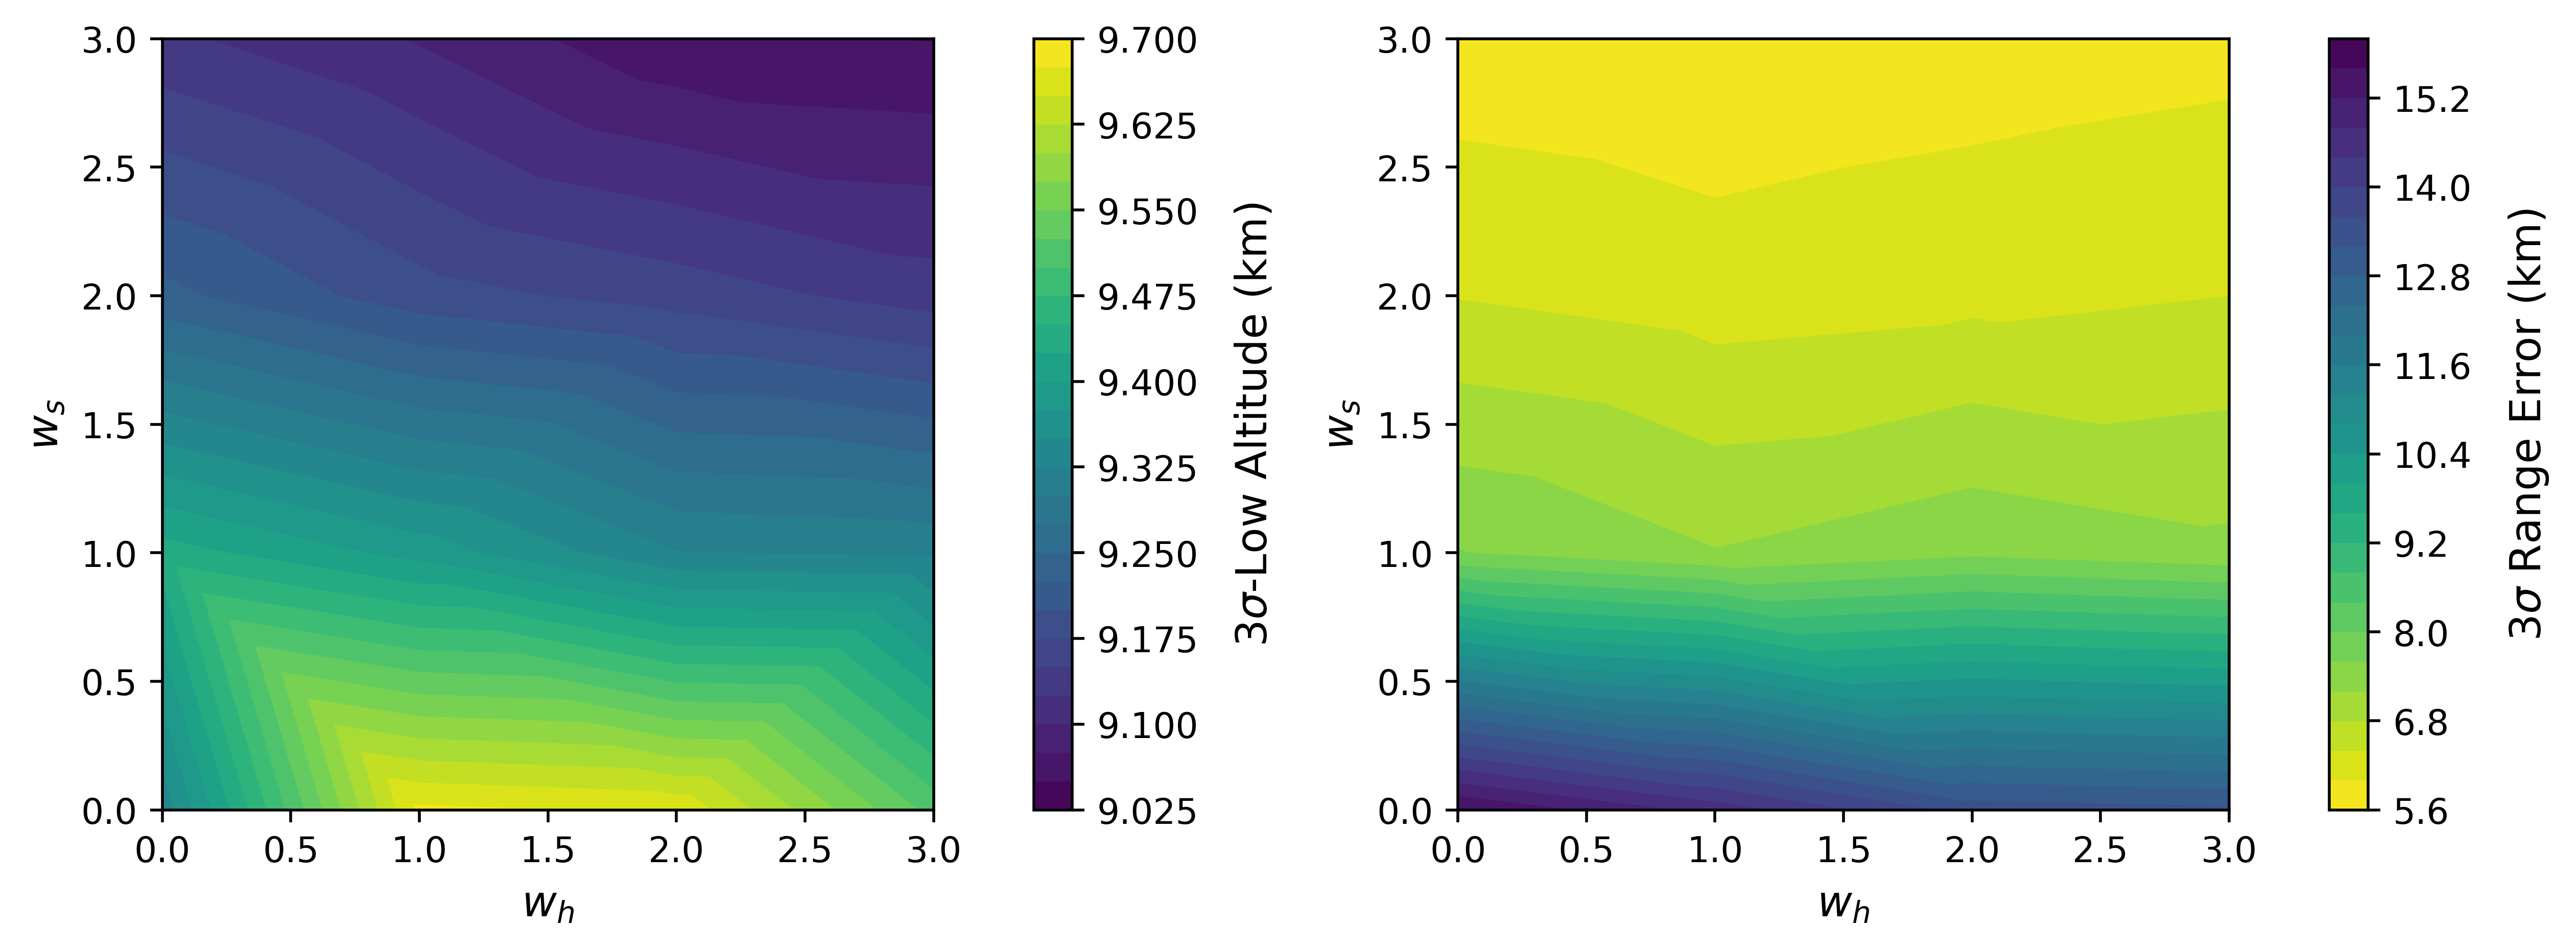
\includegraphics[width=1\textwidth]{Images/Reestimated_WeightSweepMCResults}
	\caption{}
	\label{Fig:MCResultsFixedGain}
\end{figure}
\begin{figure}[h!]
	\centering
	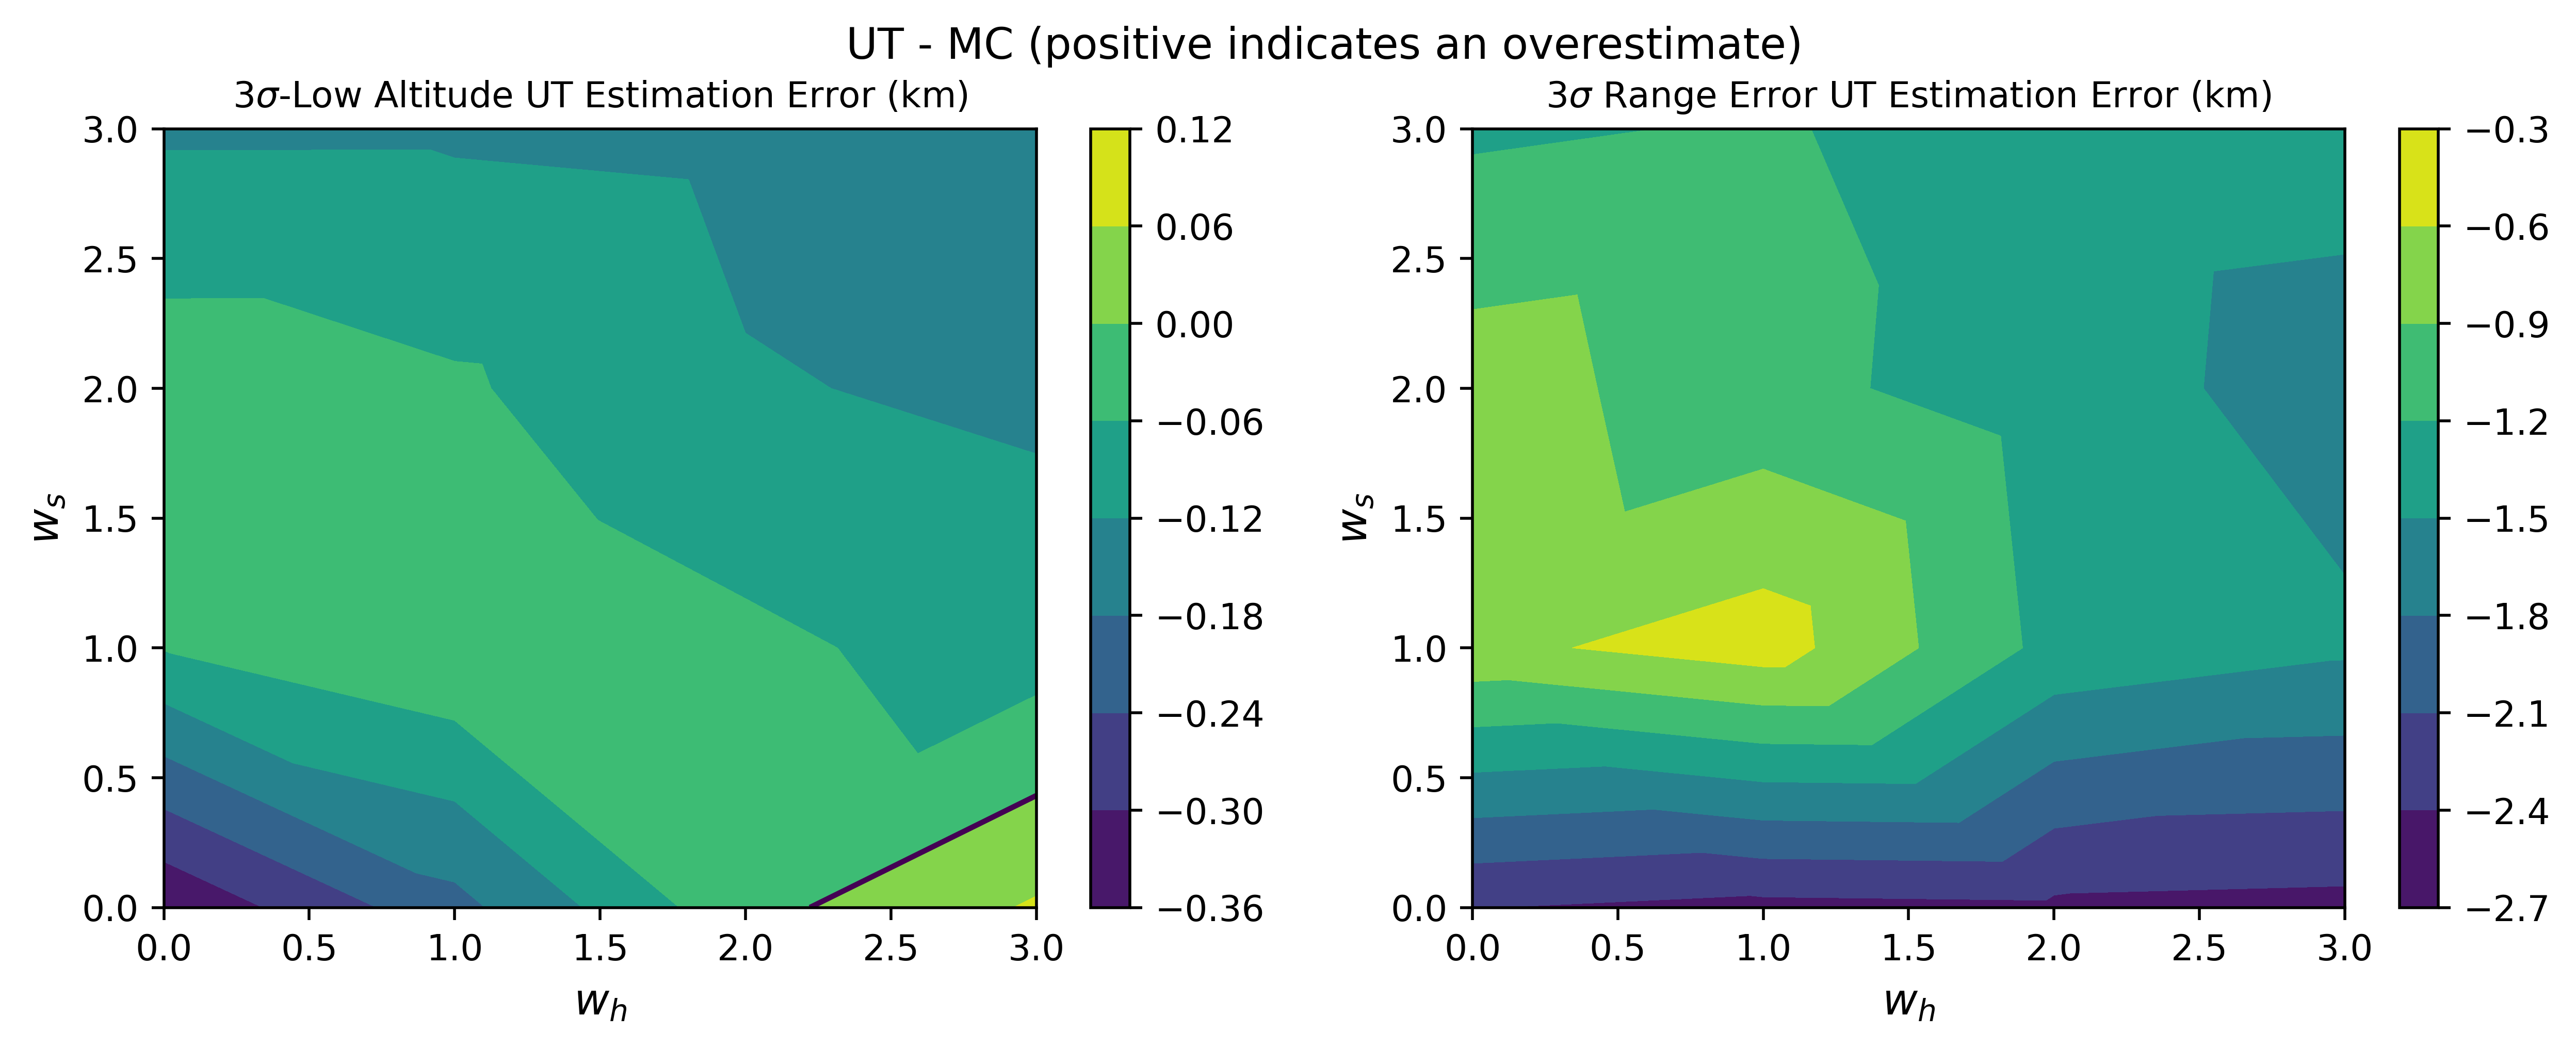
\includegraphics[width=1\textwidth]{Images/Reestimated_WeightSweepError}
	\caption{}
	\label{Fig:MCErrorsFixedGain}
\end{figure}


\section{Joint Gain Optimization}
%Motivate the constant gain optimization here by showing an example of bad MC performance when simultaneously optimizing velocity-varying gains? Then show how well the constant gains can do when jointly optimized. 

In this section, the ROGP is again solved for a variety of weights but now the gains are treated as design parameters, and the DDP modification presented in Subsection~\ref{Sec:DesignOptimization} is used to jointly optimize them alongside the reference trajectory and control. As one might intuitively expect, the effect is much more extreme with joint optimization. 

Additional 800 meters of low altitude but at the expense of a huge footprint. Similarly, very tight footprint 
\begin{figure}[h!]
	\centering
	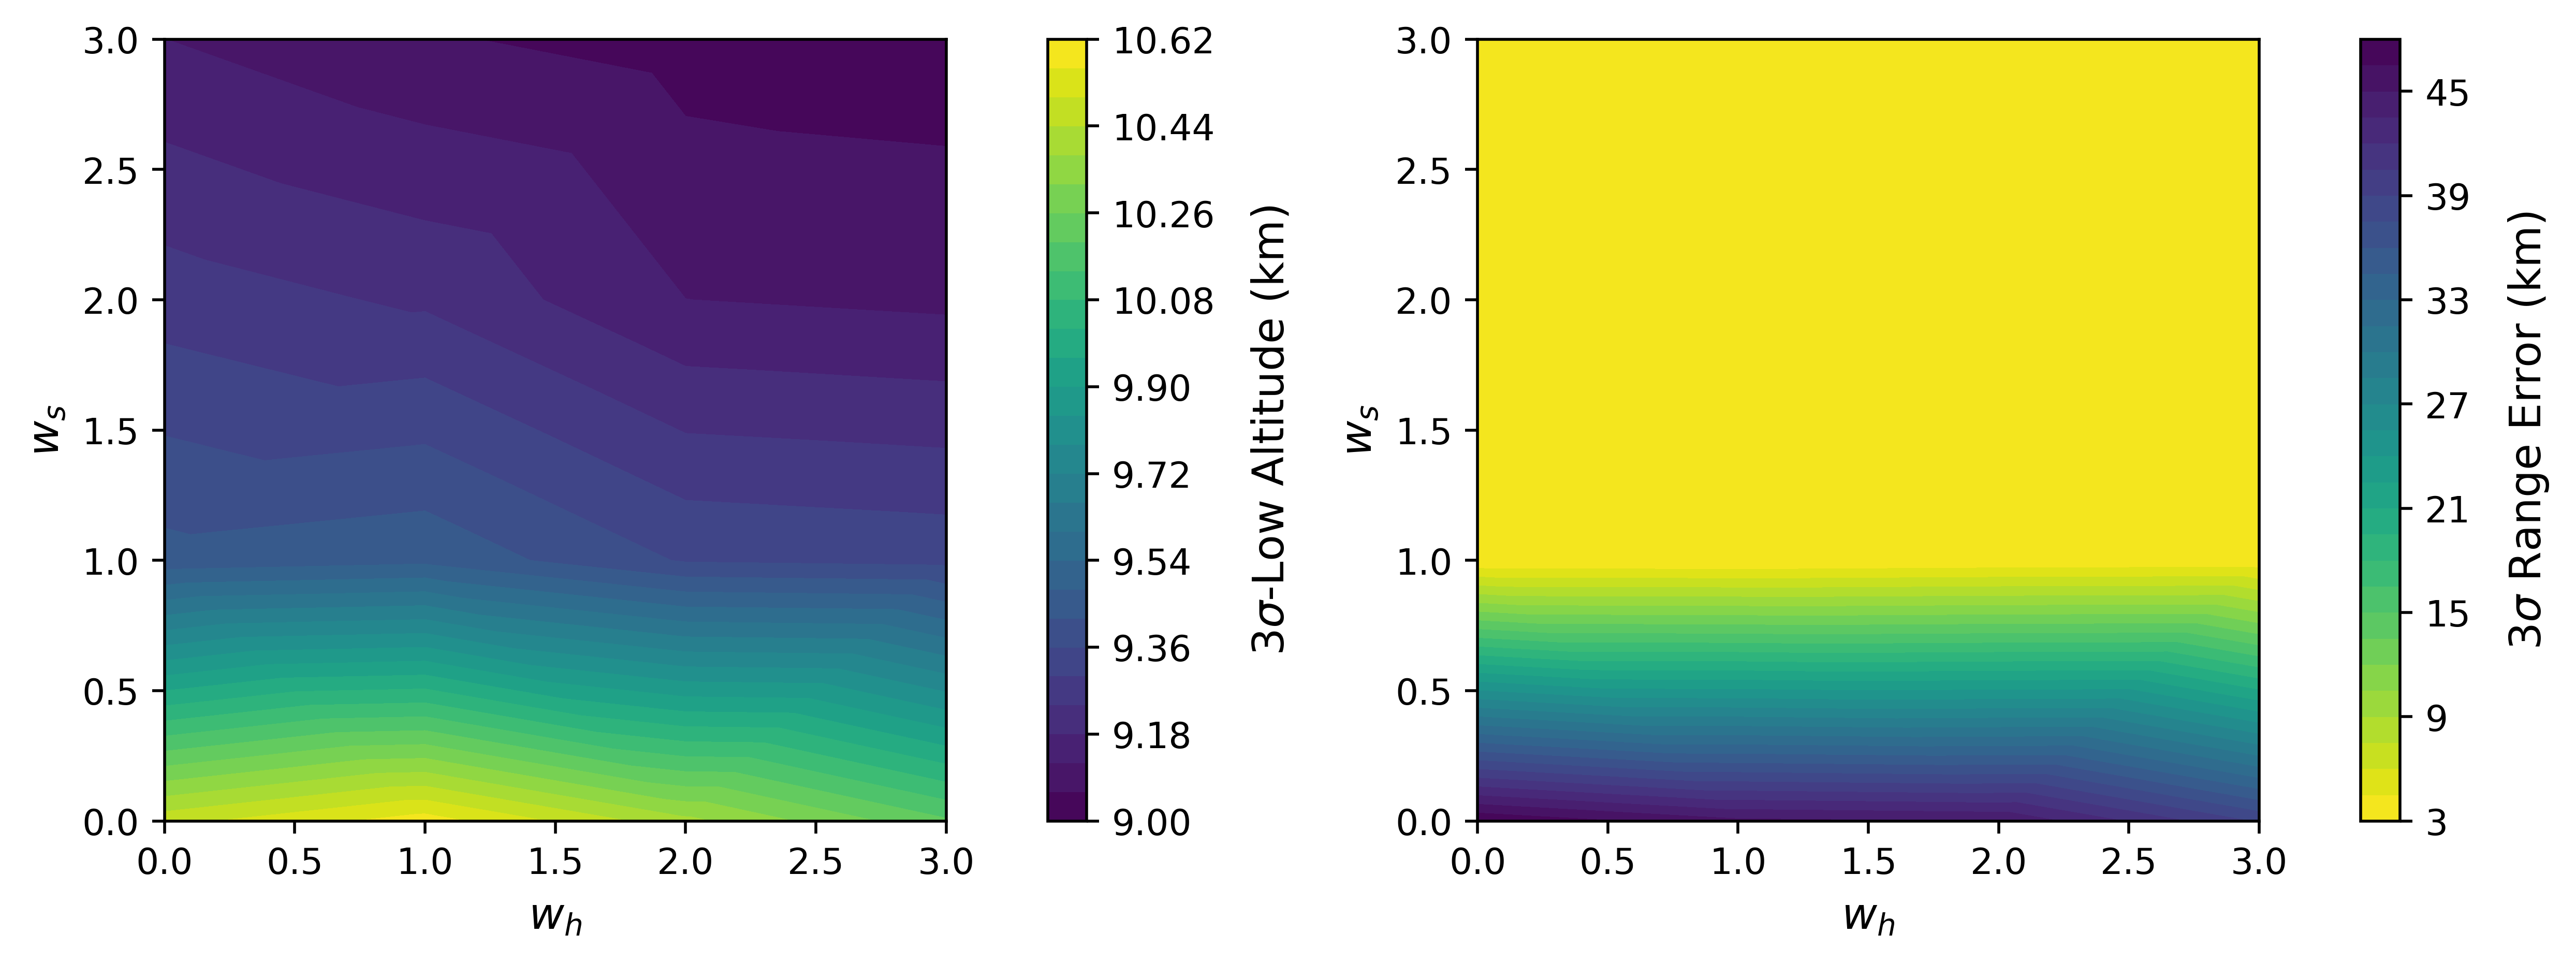
\includegraphics[width=1\textwidth]{Images/Reoptimized_WeightSweepMCResults}
	\caption{}
	\label{Fig:MCResultsOptGain}
\end{figure}
\begin{figure}[h!]
	\centering
	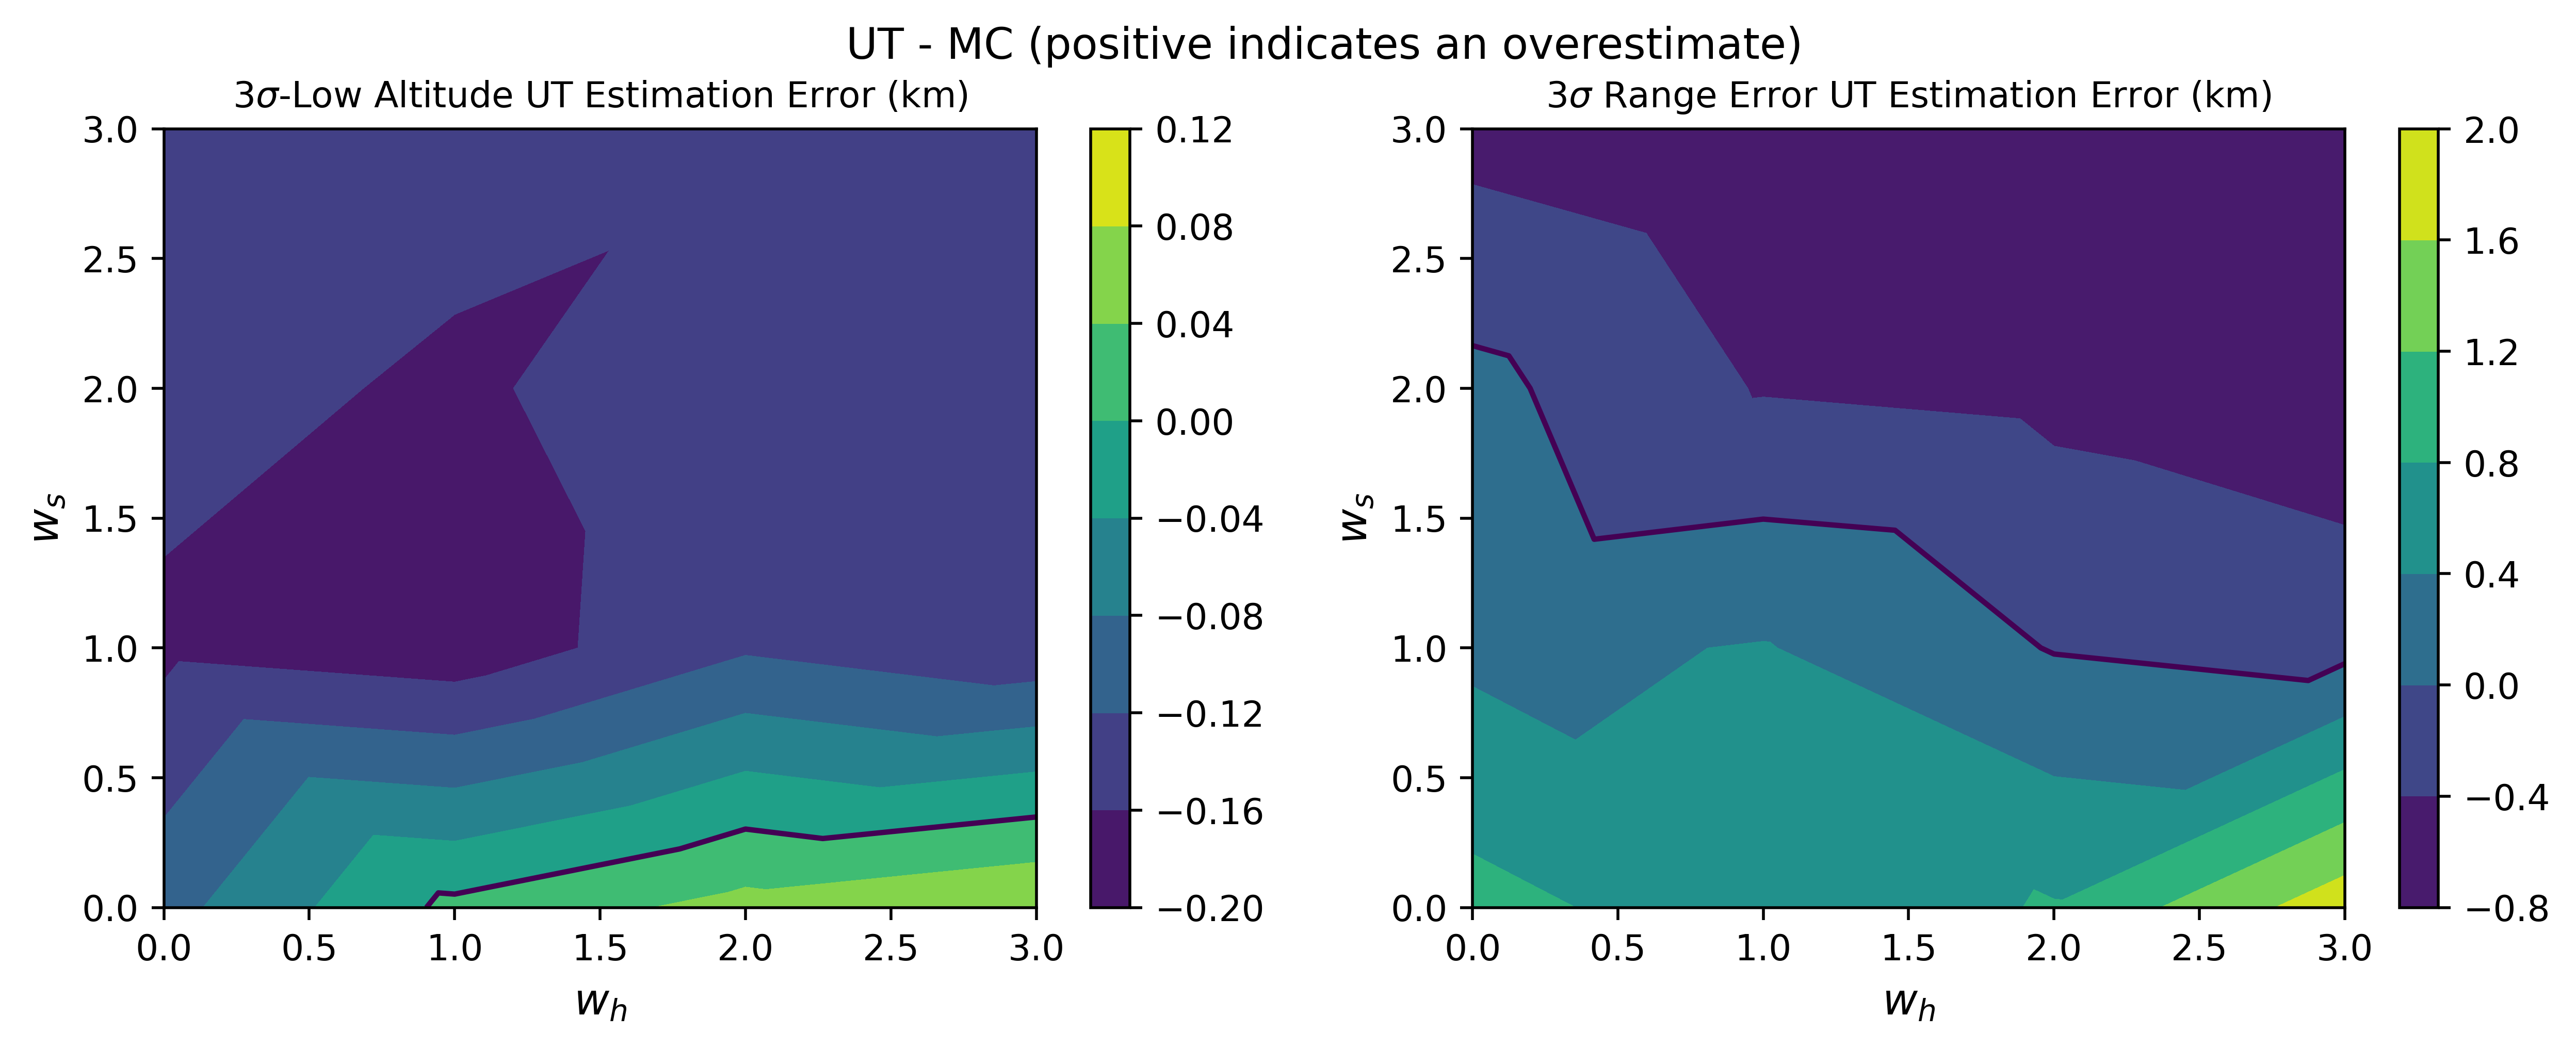
\includegraphics[width=1\textwidth]{Images/Reoptimized_WeightSweepError}
	\caption{}
	\label{Fig:MCErrorsOptGain}
\end{figure}

\section{Detailed Comparison}
Other sections are input-output, examining the tradeoffs enabled by varying the weights in the performance index. In this section we present an in-depth look at a single solution, including visualizing the samples over time. We also perform further analysis to determine which uncertainties most strongly affect performance. 

\section{As Vehicle Design Tool}
What L/D is required to achieve similar entry altitudes for a heavier vehicle of $\beta=200$? We use a simple scaling of the L/D profile $L/D$. The gains are jointly optimized, and additionally, the entry flight path angle is treated as a design variable. To estimate a useful lower bound on the L/D, we select $w_h=3, w_s=0$; the desired solution will likely place non-zero weight on the range errors, and thus need even more L/D. 
%%% Local Variables: ***
%%% mode: latex ***
%%% TeX-master: "thesis.tex" ***
%%% End: ***
